\documentclass{article}

\PassOptionsToPackage{numbers, compress}{natbib}
\usepackage{neurips_2026}

\usepackage[utf8]{inputenc}
\usepackage[T1]{fontenc}
\usepackage{amsmath,amssymb,amsfonts}
\usepackage{amsthm}
\usepackage{microtype}
\usepackage{xcolor}
\usepackage{hyperref}
\usepackage{booktabs}
\usepackage{graphicx}
\usepackage{url}
\usepackage{nicefrac}
\usepackage{algorithm}
\usepackage{algpseudocode}

\title{The Pro-Action Operator: A Scientifically-Informed, Multi-Timescale Self-Regulation Model for LLM-Agents}

\newtheorem{lemma}{Lemma}
\newtheorem{proposition}{Proposition}

\author{%
  Anonymous\thanks{Author identities withheld for double-blind review. A companion work by the same author is currently under review at a regional venue; any citation here refers to it in anonymized form.} \\
  Affiliation withheld \\
  \texttt{anonymous@institution.edu}
}

\begin{document}
\maketitle

\begin{abstract}
Contemporary LLM-agent frameworks --- ReAct, LangGraph, OpenClaw --- have prioritized \textit{capability} over \textit{motivation}, deciding \textit{when} an agent acts through exogenous flow control or task-backlog heartbeats. Homeostatic reinforcement learning (Keramati--Gutkin 2014) and active-inference agents (Friston 2017; Tschantz et al.\ 2020) internalize regulation, but often through a compact objective rather than an explicit set of delayed regulatory subsystems. However, biological regulation is not single-timescale: converging work in stress physiology, self-regulation, affect, and cognitive control treats adaptation as the interaction of subsystems --- attention, perception, hormonal (SAM adrenergic, seconds; HPA cortisol, minutes), emotional, neuropsychological, cognitive --- exchanging signals across distinct delays, consistent with the mechanism behind Yerkes--Dodson inversion and delayed reappraisal (Porcelli--Delgado 2017). We propose the \textbf{Pro-Action operator} $\Gamma$, a recursively composable, multi-timescale thermostat system. Each subsystem $k$ updates as
\[
x_{k,t+1} = x_{k,t} - \kappa_k(x_{k,t}-x^{*}_{k,t}) + \lambda_k - \alpha_k\,\rho_k(a_t,e_{t+1}) + [W\,\phi(\mathbf{x}_{t-\tau_k})]_k,
\]
with $\phi=\tanh$ elementwise, subsystem-specific delay $\tau_k$ encoding a dimensionless SAM--HPA-like ratio ($\tau_{\mathcal{H}}^{\mathrm{HPA}} \gg \tau_{\mathcal{A}}$), and action selected by an arousal-gated mixer. $\Gamma$ offers a finite, inspectable parameterization of regulation: the $\tau_k$ are explicit hyperparameters rather than hidden in orchestration depth. We specify three falsifiable properties a priori: (P1) elastic return to set-point; (P2) Yerkes--Dodson inverted-U; (P3) delayed reappraisal. As a Concept \& Feasibility contribution, the paper reports the model, a lightweight falsifiability protocol, computational sanity checks, and a completed LLM-agent benchmark. The completed benchmark shows that the operator produces opponent-discriminative behavior that exogenous-activation baselines (ReAct) and structurally similar reductions (Random-$\Gamma$, Collapse-NC) do not --- a feasibility claim, not a causal claim about the delay structure specifically.
\end{abstract}

\paragraph{Keywords.}
Homeostatic reinforcement learning; LLM agents; active inference; multi-timescale self-regulation; endogenous activation; cybernetics; self-regulation model.

\section{Introduction}

The deployment of LLM-based autonomous agents into settings of institutional consequence --- health triage, financial advice, public deliberation --- is moving faster than the science of how such agents should \textit{regulate themselves}. Whether an agent speaks, waits, defers, or escalates tends to be decided outside the agent, by an orchestrator whose control rules may be less expressive than the situations they coordinate: a small set of graph transitions, queues, or heartbeats is used to govern high-dimensional and shifting social or task states. In Ashby's terms, the controller may lack the requisite variety needed to match the variety of the environment \citep{ashby1956introduction}.

A frequently reported symptom, consistent with this variety mismatch, is the loss of activation coherence in adversarial multi-agent deliberation: floor monopolization, context collapse, and interventions that appear decoupled from any internal state the agent could be said to carry (evidence observed by the authors in a companion work, currently under review). The pattern suggests that \textit{when} an agent acts may depend on structure the dominant paradigm does not explicitly represent.

Contemporary LLM-agent frameworks --- ReAct, LangGraph, OpenClaw --- have prioritized \textit{capability} (what an agent can do) over \textit{motivation} (why and when it should act at all), addressing activation via cognitive while-loops and exogenous flow control. Homeostatic reinforcement learning (Keramati--Gutkin 2014) and active-inference agents (Friston 2017; Tschantz et al.\ 2020) internalize regulation, but do not provide a compact LLM-agent operator in which attention, interoception, emotion, memory, cognition, and stress-like physiology are all explicit delayed regulators. Intelligent animals, including humans, regulate behavior through multiple interacting systems --- attention, arousal, affect, memory, deliberation --- operating on distinct timescales whose relative priority shifts with context; dominant LLM-agent paradigms treat activation as a single-objective signal or exogenous flow control.

The problem is older than LLM-agents. Mid-20th century behaviorism defined it precisely by bracketing it: the stimulus--response mapping could be studied scientifically because the intervening machinery --- the \textit{black box} --- was deliberately left unspecified. Decades of subsequent research opened that box from different angles: behavioral biology established that animal regulation is multi-drive and hierarchical; stress physiology revealed fast (adrenergic, seconds) and slow (cortisol, minutes) adaptation axes with distinct roles; affective neuroscience showed that emotion is not an output label but a construction that shapes perception, memory, and action; evolutionary game theory demonstrated that social behavior is governed by reciprocity and temporal discounting, not instantaneous utility; cybernetics formalized why a regulator must match the variety of what it controls. Each tradition contributed a piece. Nobody has assembled these threads for LLM-agents into a single, compact, falsifiable operator. Section~\ref{sec:related} reviews each contribution in detail. Opening the black box matters beyond mechanistic completeness: (i) $\Gamma$ provides a finite, inspectable state vector, making each subsystem's contribution auditable rather than buried in prompt engineering; (ii) a controller tracking regulatory state creates the precondition for agents that adapt to their own arousal trajectory; (iii) explicit emotional and hormonal channels provide the computational substrate for empathy modeling --- recognizing a counterpart's affective state --- which is structurally distinct from fine-tuning on empathy datasets.

What remains comparatively unexplored is a single, computable, falsifiable operator that integrates these disciplinary insights for LLM agents. The central biological clue is that regulation is not a single controller but a \textit{system of subsystems} --- attention, perception, hormonal (SAM adrenergic, seconds; HPA cortisol, minutes), emotional, neuropsychological, cognitive --- exchanging signals across distinct delays. The SAM--HPA timescale split is not decorative: it is consistent with the mechanism behind Yerkes--Dodson inversion, post-stress reappraisal windows, and delayed-valuation shifts \citep{porcelli2017stress}. The scientific question is therefore whether activation itself can be treated as a regulated internal process --- a coupled set of thermostat-like variables whose delayed interactions determine when the agent should speak, wait, defer, or escalate --- and whether the smallest such structure remains distinguishable from a single-timescale regulator.

We propose the \textbf{Pro-Action operator} $\Gamma$ as a model, not an experimental technique. $\Gamma$ treats activation as a recursively composable system of six coupled thermostats with explicit update delays. The contribution type is Concept \& Feasibility: the idea is intentionally broader than what can be validated in a single benchmark, but it must still be made operational enough to fail. The contributions of this paper are primarily \textit{modeling}: (i) a formal operator integrating multi-timescale regulation; (ii) the framing of $\Gamma$ as a Self-Regulation Model (SRM) class complementary to capability-oriented LAMs; (iii) an a priori specified falsifiability protocol; (iv) a reference implementation checked by computational sanity tests; and (v) a preliminary LLM-agent benchmark snapshot used as feasibility evidence rather than final empirical adjudication.

\section{Related work}\label{sec:related}

\paragraph{LLM-agent orchestration.} Recent LLM-agent frameworks such as ReAct \citep{yao2023react}, LangGraph, and OpenClaw made language models operational by embedding them in action loops, tool graphs, and multi-agent workflows. This was a necessary engineering step: without explicit structure, an LLM has no durable procedure for acting in an environment. More recently, agent architectures have incorporated persistent memory streams, reflection, and simulated affective states to enrich the content of decisions \citep{park2023generative,kaiya2023lyfe,wang2023emotional,wang2023voyager}. The limitation common to both generations is that activation is usually externalized: the graph or supervisor decides when the model acts; the model supplies content for that externally selected moment. $\Gamma$ is complementary: those works provide richer \textit{content}; $\Gamma$ provides a principled internal account of \textit{timing}.

\paragraph{Internal regulation across timescales.} A different tradition begins from the opposite assumption: action should be driven by an internal regulatory state. Homeostatic RL makes internal deficit part of the reward \citep{keramati2014homeostatic}; active inference gives a broader variational formulation \citep{friston2017active,parr2022active}. These approaches are important --- they move regulation inside the agent --- but do not yield a compact operator with separately inspectable subsystem delays. Once regulation is internalized, the next question is whether a single regulatory signal is sufficient. Stress physiology and allostasis suggest it is not: fast sympathetic responses (SAM, seconds) and slower endocrine/cognitive recovery (HPA, minutes) play distinct adaptive roles \citep{sterling1988allostasis,mcewen2007physiology,kirschbaum1993cortisol}. The remaining question is which internal variables deserve to be modeled. Interoceptive and somatic-marker accounts connect bodily state to action readiness \citep{damasio1994descartes,craig2009you}; affect-regulation accounts treat emotion as part of how situations are appraised \citep{barrett2017how,ledoux2015rethinking}; evolutionary game theory adds reciprocity and temporal discounting as social constraints \citep{nowak2006evolutionary,henrich2005foundations}. Together, these literatures motivate attention, interoception, emotion, memory, cognition, and hormonal dynamics as functional regulators rather than decorative modules.

\paragraph{Systems, cybernetics, and the gap.} If these variables are treated as separate regulators, the final problem is structural: how should they be composed? Cybernetics supplies the relevant language: Ashby's law of requisite variety requires a regulator rich enough to match the environment \citep{ashby1956introduction}; Beer's Viable System Model adds recursive organization \citep{beer1972brain}; systemism frames the relevant object as composition rather than isolated component \citep{bunge2003emergence,romero2018scientific}. The gap might be narrow yet important. To our knowledge, the threads above --- exogenous orchestration, homeostatic internalization, multi-timescale physiology, affect regulation, and cybernetic composition --- have not been combined into a small, falsifiable LLM-agent operator in which the six regulatory domains are explicit state variables with explicit delays. That is the gap $\Gamma$ is designed to occupy.

\section{The Pro-Action operator}

\subsection{Axioms of homeostatic autonomy (A1--A9)}

Before defining $\Gamma$, we make explicit the modeling commitments that the operator assumes. The axioms are not empirical results or theorems; they state, in this model, what counts as an autonomous, self-regulating agent, which internal variables are allowed to regulate action, and how those variables may be composed. This is meant to avoid leaving the agent's ontology implicit in implementation choices. The axiom set was subjected to a formal coherence check using SMT-based tools (Z3) to verify that no pair of axioms is mutually contradictory under the intended semantics; all checks passed.

We extend the Axioms of Homeostatic Autonomy from the companion work (A1--A3) with six additional axioms that make the multi-timescale structure explicit:

\textbf{A1--A3 (Kernel).} Autonomy, Impulse, and Quality Gate: the agent maintains an internal deficit $\delta_i$ that drives action probability $p_i(t) = \sigma(D(\delta_i(t)))$, reduced by action quality $g$.

\textbf{A4 (Perception as initial appraisal).} Every stimulus is appraised before selective attention. A perception operator $\mathcal{P}$ produces an initial situational appraisal $\tilde o_t = \mathcal{P}(o_t, \mathcal{I}_t, \mathcal{M}_t; x_{\mathcal{P},t})$, encoding what the stimulus means independent of current priorities.

\textbf{A5 (Attention as saliency gate).} Not every appraised feature enters the action-selection context. An attention operator $\mathcal{A}$ filters the perceived signal, selecting $o'_t = \mathcal{A}(\tilde o_t, \mathcal{D}_t, \mathcal{M}_t; x_{\mathcal{A},t})$ based on current drives and memory. Interoceptive signals $\mathcal{I}_t$ feed in parallel to both $\mathcal{P}$ and $\mathcal{A}$.

\textbf{A6 (Memory as ubiquitous prior).} A state $\mathcal{M}_t$ biases all subsystems and updates post-action.

\textbf{A7 (Drives as set-point generators).} Set-points are not constants: $\mathbf{x}^{*}_t = \mathcal{D}_t$.

\textbf{A8 (Fast/slow parallelism with arbitrator).} Two routes produce action candidates $c^{\text{fast}}$, $c^{\text{slow}}$; an arbitrator assigns precision weights $\pi_{\text{fast}}$, $\pi_{\text{slow}}$.

\subsection{The operator}

\begin{figure}[t]
\centering
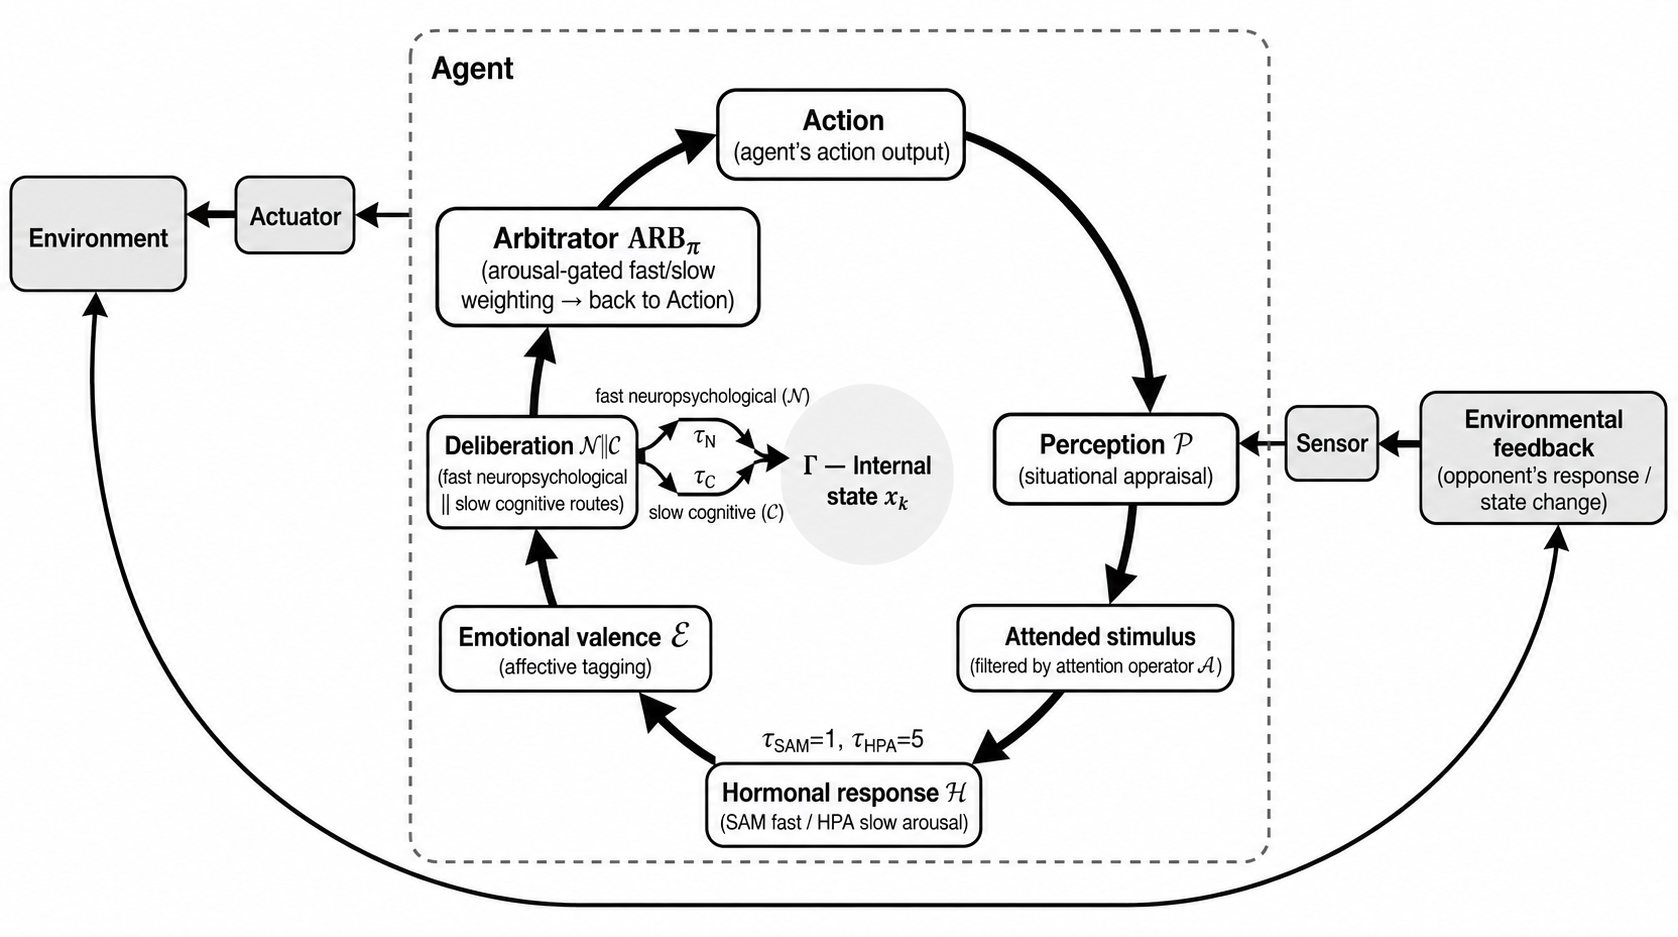
\includegraphics[width=0.72\linewidth]{figures/fig_arch.png}
\caption{The Pro-Action operator $\Gamma$: regulatory cycle in canonical clockwise order. Perception ($\mathcal{P}$, situational appraisal) feeds Attention ($\mathcal{A}$, saliency filtering), which gates the Hormonal arousal module ($\mathcal{H}$, SAM fast / HPA slow), Emotional valence ($\mathcal{E}$), and a Deliberation gate routing to the Neuropsychological fast path ($\mathcal{N}$, $\tau_\mathcal{N}$) or Cognitive slow path ($\mathcal{C}$, $\tau_\mathcal{C}$); the Arbitrator ARB$_\pi$ applies arousal-gated weighting before action emission. Notation: $\circ$ denotes composition, $\|$ parallel evaluation (routes merged by ARB$_\pi$), and $\mathcal{O}[\cdot]$ the output projection selecting the final action.}
\label{fig:arch}
\end{figure}

We define $\Gamma$ as the composition (Figure~\ref{fig:arch}):
\begin{equation}
\Gamma := \mathcal{O}\Big[\text{ARB}_\pi\Big(\underbrace{(\mathcal{N}_{\text{fast}}\circ\mathcal{H}_{\text{SAM}})}_{\text{fast route}} \big\| \underbrace{(\mathcal{C}\circ\mathcal{E}\circ\mathcal{A}\circ\mathcal{P})}_{\text{slow route}} \Big)\Big]\Big|_{\mathcal{I},\,\mathcal{M},\,\mathcal{D}}
\end{equation}

Each subsystem $k$ updates as:
\begin{equation}\label{eq:master}
\boxed{x_{k,t+1} = x_{k,t} - \kappa_k(x_{k,t}-x^{*}_{k,t}) + \lambda_k - \alpha_k\,\rho_k(a_t,e_{t+1}) + [W\,\phi(\mathbf{x}_{t-\tau_k})]_k}
\end{equation}
with $\phi = \tanh$ elementwise. The delays $\tau_k$ are dimensionless non-negative integers (in agent-interaction rounds), not literal biological durations; what the model inherits from SAM--HPA physiology is the \emph{ratio} $\tau_{\mathcal{H}}^{\mathrm{HPA}} \gg \tau_{\mathcal{A}}$, not the absolute timescales. Action is selected by:
\begin{equation}\label{eq:mixer}
a^{*}_{t+1} = \arg\min_a\; \pi_f\,\mathcal{F}_{\text{short}} + (1-\pi_f)\,\mathcal{F}_{\text{long}} + \gamma\|Q^{1/2}(\mathbf{x}_{t+1}(a) - \mathbf{x}^{*}_{t+1})\|^2, \quad \pi_f = \sigma(c \cdot x_{\mathcal{H}} + b)
\end{equation}
where $\mathbf{x}_{t+1}(a)$ denotes the predicted next state under candidate action $a$, depending on $a$ through the action-quality term $\rho_k(a, e_{t+1})$ in Eq.~\eqref{eq:master} --- it is this dependence that makes the homeostatic deficit penalty action-relevant. $\mathcal{F}_{\text{short}}$, $\mathcal{F}_{\text{long}}$ are generic cost functionals inspired by expected-free-energy control over horizons $h_s \ll h_l$, and $Q \succeq 0$ is a diagonal precision matrix (distinct from the coupling matrix $W$ in Eq.~\eqref{eq:master}). In the IPD instantiation below we do not claim a strict active-inference implementation with an explicit generative model. The mixer is not literally executed as an argmin over LLM completions: the controller modulates the prompt seen by the LLM (Section~\ref{sec:prompt-protocol}) and the LLM emits the action; Eq.~\eqref{eq:mixer} is the compact controller-level expression of fast/slow arbitration that the prompt encodes.

\subsection{Non-absorption of delay parameters}

\begin{proposition}[Non-absorption of delays]\label{prop:nonabsorption}
Let $\Gamma_\tau$ denote Eq.~\eqref{eq:master} with delays $\boldsymbol{\tau} = (\tau_1,\dots,\tau_6) \in \mathbb{Z}_{\geq 0}^6$ and coupling matrix $W \neq \mathbf{0}$. For any two delay vectors $\boldsymbol{\tau} \neq \boldsymbol{\tau}'$ with $\tau_k \neq \tau_k'$ for at least one $k$ such that $[W]_{k,\cdot} \neq \mathbf{0}$, there is no reparametrization $(\kappa_k',\lambda_k',\alpha_k')$ of the non-delayed terms that makes the impulse-response of $\Gamma_{\tau'}$ identical to that of $\Gamma_\tau$. Equivalently, $\tau_k$ is not absorbable into $(\kappa_k,\lambda_k,\alpha_k)$.
\end{proposition}

The argument (Appendix~\ref{app:proof}) is an order-mismatch in the discrete-time z-domain: a delayed subsystem has transfer-function denominator degree $\tau_k+1$, enforcing $\tau_k$ zero-output samples by causality that no delay-free reparametrization can replicate. This establishes that $\tau_k$ is identifiable from observed trajectories and that $\Gamma$ occupies a distinct model class from any delay-free parametrization of the same dimension.

\subsection{Reductions to simpler models}

\textbf{Reduction to Driveplexity.} Driveplexity (companion work, currently under review) is a single-drive homeostatic activation model in which each LLM-agent maintains a scalar epistemic deficit $\delta_i$ that decays at a fixed rate and is reduced by the quality of each action executed. $\Gamma$ subsumes it: when $x_{\mathcal{A}} = \dots = x_{\mathcal{N}} \equiv 0$, $\mathcal{A}=\text{id}$, $\mathcal{I}=\mathcal{M}=\mathcal{D}=\emptyset$, $\pi_{\text{fast}}\equiv 0$, $W=\mathbf{0}$, $\kappa_{\mathcal{C}}=0$, and $\mathbf{x} \to x_{\mathcal{C}} \equiv \delta_i$, Equation~\eqref{eq:master} reduces to $\delta_{t+1} = \delta_t + \lambda - \alpha \cdot g(e^{(t)}, e^{(t+1)})$, which is exactly A1--A3.

\textbf{Reduction to homeostatic RL.} When $\boldsymbol{\kappa}=\mathbf{0}$ and all $\tau_k=0$, $\Gamma$ becomes a reactive drive-based policy consistent with the simplified form of Keramati--Gutkin (2014).

The six-subsystem partition is motivated by six regulatory functions that each relevant literature distinguishes independently. Whether five suffice is tested empirically by the Collapse-NC ablation, which merges $\mathcal{N}$ and $\mathcal{C}$ into a single regulator: the completed benchmark shows Collapse-NC produces a flat opponent profile (Grim cooperation 0.829, range 0.032) comparable to Random-$\Gamma$ (0.843, range 0.017), suggesting the $\mathcal{N}$--$\mathcal{C}$ partition is load-bearing rather than over-parameterized.

\section{Falsifiability protocol}

To avoid the vacuity of untestable models, three properties are specified a priori before any experiment:

\textbf{(P1) Elastic return to set-point.} Under perturbation, each $x_k$ returns to $x^{*}_k$ with measurable half-life $t_{1/2}$.

\textbf{(P2) Yerkes--Dodson inverted-U.} Arousal vs. performance follows an inverted-U; ablation of SAM coupling ($\mathcal{H}_{\text{SAM}}$) collapses it to monotone. Target BFI $\geq 0.70$ against Porcelli--Delgado (2017).

\textbf{(P3) Delayed reappraisal.} Cross-lag correlation between $x_{\mathcal{C}}$ and $x_{\mathcal{E}}$ peaks at lag $\tau_{\mathcal{H}}^{\mathrm{HPA}}$.

\subsection{Behavioral Fidelity Index (BFI)}

\begin{equation}
\mathrm{BFI} = \exp\bigl(-W_1(\mu_{\text{agent}}, \mu_{\text{human}})/\lambda\bigr)
\end{equation}
over-normalized marginals of cooperation rate, action volatility, and log-response-time proxy. The response-time proxy is an engineering observable, not a claim of equivalence to human decision time. The model is supported if BFI exceeds thresholds on $\geq 2$ of 3 properties and the corresponding ablation degrades the property.

\subsection{Experimental design}

We test $\Gamma$ within the Iterated Prisoner's Dilemma (IPD). The reason for this choice is that IPD has extensive empirical evidence of human behavior in repeated social interaction \citep{axelrod1984evolution,nowak2006evolutionary,porcelli2017stress}, providing a non-trivial baseline for comparing agent behavior against human patterns. The setting we establish for the game is 10\% noise and 50 rounds, with a forced-defection perturbation at round 10 to test the elastic-return property (P1) by creating a measurable deviation from the set-point. Sotopia-derived deliberation \citep{zhou2024sotopia} is deferred to future work because it is better suited for ecological validity than for the first controlled falsification of the operator.

Baselines serve two purposes: ReAct represents the dominant exogenous-activation paradigm; HRRL (homeostatic-RL reduction) and Drive-only (pure controller, no LLM) test whether $\Gamma$ adds value beyond a single-drive or LLM-free controller.

Three instruction-tuned LLM providers are used as policy-execution layers: OpenAI (\texttt{gpt-5-nano}), Anthropic (\texttt{claude-haiku-4-5}), and DeepSeek (\texttt{deepseek-v4-flash}). These models were selected as the comparable lite/flash/nano variants of each provider's frontier line—well benchmarked and roughly matched in capability tier. Using three independent providers reduces the controller-level findings' dependence on any single provider's instruction-tuning regime. Each provider/model is held fixed across conditions, so that within-provider contrasts isolate the controller rather than model identity. Provider-level summaries are reported as diagnostics, not as claims about provider quality.

\textbf{Inference parameters.} OpenAI \texttt{gpt-5-nano} uses default temperature with a per-round seed for reproducibility; Anthropic \texttt{claude-haiku-4-5} uses temperature $0$ and \texttt{max\_tokens} $512$ (no seed parameter exposed); DeepSeek \texttt{deepseek-v4-flash} uses temperature $0$ and \texttt{max\_tokens} $512$. Calls return JSON objects; OpenAI and DeepSeek use \texttt{response\_format: json\_object}. Concurrency is capped at $8$ in-flight cells per provider, with up to $4$ exponential retries on transient errors.

All frozen constants are assigned a provenance category before evaluation (Table~\ref{tab:params}). Values marked as smoke-test calibration were chosen before the LLM benchmark to satisfy non-divergence, set-point return, and visible perturbation response in the numerical simulator; final reporting will include sensitivity checks for critical constants.

\begin{table}[h]
\caption{Frozen parameter provenance for the IPD instantiation. Index mapping: 0=Perception, 1=Attention, 2=Hormonal (SAM), 3=Hormonal (HPA), 4=Neuropsychological, 5=Cognitive.}
\label{tab:params}
\centering
\begin{tabular}{lll}
\toprule
Parameter & Value & Provenance \\
\midrule
$\boldsymbol{\lambda}$ & $[.08,.07,.10,.08,.06,.10]$ & smoke-test calibration \\
$\boldsymbol{\alpha}$ & $[.20,.15,.25,.20,.10,.15]$ & smoke-test calibration \\
$\boldsymbol{\kappa}$ & $[.10,.10,.15,.12,.08,.10]$ & smoke-test calibration \\
$\mathbf{x}^{*}$ & $[.3,.2,.3,.1,.2,.4]$ & principled prior / stable interior set-point \\
$\tau_{\mathrm{SAM}},\tau_{\mathrm{HPA}}$ & $1,5$ rounds & dimensionless fast/slow ratio \\
$W$ & sparse signed coupling matrix & functional constraint and ablation interpretability \\
$Q$ & $I_6$ (identity) & smoke-test calibration; precision matrix in Eq.~\eqref{eq:mixer} \\
Rounds & 50 & comparability requirement for final cells \\
\bottomrule
\end{tabular}
\end{table}

Seven ablation conditions (Table~\ref{tab:ablaciones}) isolate the contribution of the main regulatory components. Full-$\Gamma$ uses all six thermostats in the canonical order: Perception (appraisal) $\to$ Attention (saliency filtering) $\to$ Emotional (valence) $\to$ Hormonal (arousal, fast-slow routes) $\to$ Neuropsychological and Cognitive (deliberation routes in parallel) $\to$ Arbitrator (weighting). No-$\mathcal{H}$ removes the hormonal channel (both SAM and HPA); No-$\mathcal{E}$ neutralizes emotional valence; No-$\mathcal{N}$ removes the slow neuropsychological route. Random-$\Gamma$ permutes the entries of $W$ while preserving all other parameters --- same six thermostats, same $\tau_k$, same hyperparameters, but biologically-unmotivated wiring --- to isolate the contribution of the coupling structure rather than parameter count. Collapse-NC merges the neuropsychological ($\mathcal{N}$) and cognitive ($\mathcal{C}$) subsystems into a single regulator by averaging their parameters and symmetrizing their $W$ rows and columns, testing whether the 6-subsystem partition is necessary or whether 5 would suffice.

\begin{table}[h]
\caption{Ablations. Full-$\Gamma$ uses all six thermostats; ablations remove, permute, or collapse selected regulatory components.}
\label{tab:ablaciones}
\centering
\small
\resizebox{\linewidth}{!}{%
\begin{tabular}{lp{6cm}l}
\toprule
Condition & Change from Full-$\Gamma$ & Purpose \\
\midrule
Full-$\Gamma$ & --- & Reference \\
No-$\mathcal{H}$ & Hormonal channel ($\mathcal{H}_{\text{SAM}}$, $\mathcal{H}_{\text{HPA}}$) zeroed & Fast-timescale contribution \\
No-$\mathcal{E}$ & Emotional valence zeroed & Affect as stabilizer vs.\ noise \\
No-$\mathcal{N}$ & Neuropsychological channel zeroed & Slow deliberation contribution \\
Random-$\Gamma$ & $W$ entries permuted; $\tau_k$, $\kappa$, $\lambda$, $\alpha$ unchanged & Biologically-motivated wiring vs.\ parameter count \\
Collapse-NC & $\mathcal{N}$ and $\mathcal{C}$ merged into one regulator & 6-subsystem vs.\ 5-subsystem partition \\
\bottomrule
\end{tabular}}
\end{table}

\subsection{Prompt protocol and label-priming control}\label{sec:prompt-protocol}

The controller modulates the LLM through a frozen, version-controlled prompt template: each round, the six thermostat values $\mathbf{x}_t$ and the aggregated proposal $p_C, h_{\mathrm{SAM}}$ are inserted with semantic anchors pairing each value with its set-point and a qualitative low/high interpretation (e.g., \texttt{hormonal = 0.58 (set-point 0.30; low = calm, high = elevated arousal)}). The LLM may follow or override $p(C)$; the controller modulates rather than mandates. A pre-specified \emph{scrambled-labels} control arm (semantic labels permuted to neutral identifiers while numeric values remain bound to their subsystem) is reserved for the post-completion ancillary analysis. Full implementation details are in the open repository.

\section{Preliminary verification}

Before empirical evaluation, we subjected Equation~\eqref{eq:master} and its reference implementation to computational sanity checks using symbolic algebra (SymPy), SMT-based counterexample search (Z3), arbitrary-precision arithmetic (mpmath), and numerical dynamical tests (NumPy). These checks are not a formal verification of the scientific model. They test internal consistency: whether the implementation preserves the intended update structure, avoids immediate numerical divergence, and contains Driveplexity as a reduction.

\textbf{Smoke-test results (all pass):} (1) Set-point convergence: $\|\mathbf{x}_t - \mathbf{x}^{*}\| < 0.15$ after 10 rounds. (2) Elastic return half-life $t_{1/2} = 3.2$ rounds. (3) $\pi_{\text{fast}}$ rises from 0.35 to 0.92 under threat. (4) 20 iterations without divergence. (5) Driveplexity is an invariant subspace of $\Gamma$ ($\delta = -0.0513$).

\textbf{Simulation trajectories.} Figure~\ref{fig:thermostats} shows the six thermostat trajectories for two agents over 30 rounds. Both agents converge toward their set-points ($\mathbf{x}^{*} = [0.3, 0.2, 0.3, 0.1, 0.2, 0.4]$) despite perturbation at round 10 (forced defection).

\begin{figure}[h]
\centering
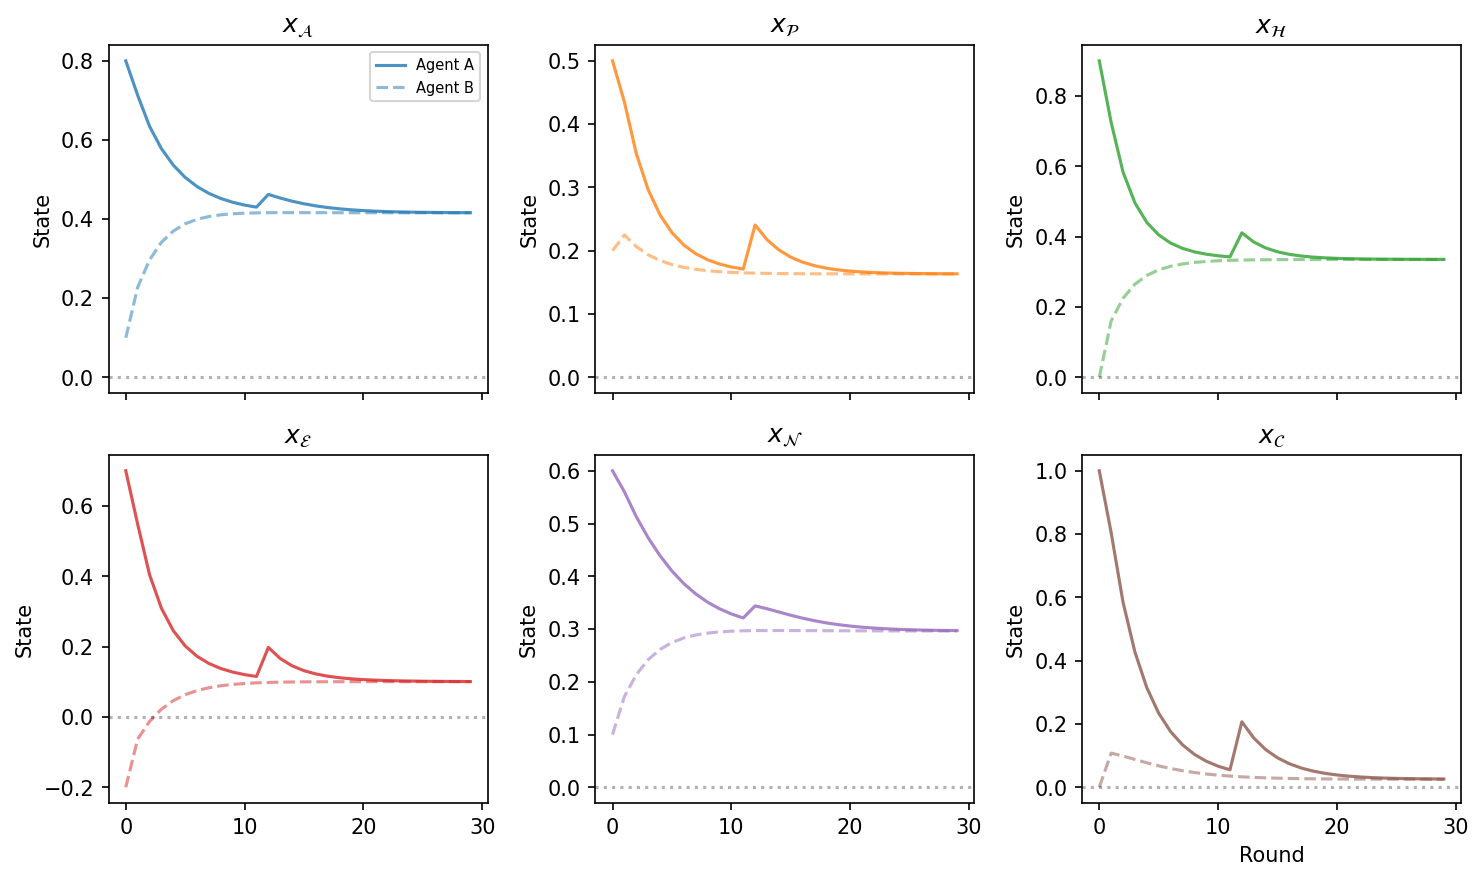
\includegraphics[width=\linewidth]{figures/fig1_thermostats.png}
\caption{Subsystem thermostat trajectories for two agents in IPD with noise. The perturbation at round 10 (forced defection) triggers a transient deviation, followed by an elastic return toward set points.}
\label{fig:thermostats}
\end{figure}

Cumulative payoffs and the P1 elastic-return zoom on $x_{\mathcal{H}}$ are provided in Appendix~\ref{app:sensitivity} (Figures~\ref{fig:payoffs} and \ref{fig:elastic}). These results verify the \textit{internal consistency} of the dynamics, not biological or behavioral fidelity. Parameter sensitivity checks (Appendix~\ref{app:sensitivity}) confirm that P1 elastic return is robust to $\pm 20\%$ uniform scaling of $\kappa$ and $\lambda$, indicating that the smoke-test calibration point is not isolated.

\subsection{Interim LLM-agent benchmark snapshot}

We then asked whether the operator remains meaningful when the policy-execution layer is no longer a numerical mock agent but a real LLM prompted to play the Iterated Prisoner's Dilemma under a frozen controller state. Each \emph{cell} denotes an independent experimental unit: a tuple (\mbox{$\Gamma$-condition} $\times$ provider $\times$ opponent $\times$ seed) run for 50 IPD rounds. The benchmark is now fully covered: all 920 cells have completed 50 rounds with balanced opponent coverage. All seven LLM conditions and two numerical reductions reach 120 and 40 cells respectively, each balanced across three providers and four opponent policies. The results below constitute the completed feasibility assessment.

The first useful sign is that Full-$\Gamma$ does not collapse to a trivial policy. Mean cooperation is 0.720 (sd 0.165, 95\% CI [0.690, 0.749]; 10k bootstrap resamples), with action volatility of 16.0 switches per 50-round cell (95\% CI [15.0, 17.0]). Opponent sensitivity is preserved and notably discriminative: Full-$\Gamma$ cooperates more with TFT (0.827) and GTFT (0.839), less with Grim (0.495), and intermediately with Random (0.719). The contrast with Random-$\Gamma$ (120 balanced cells) is informative: a randomly-wired controller cooperates uniformly across all opponents --- TFT 0.839, GTFT 0.828, Grim 0.843, Random 0.845 --- producing nearly flat opponent sensitivity (range 0.017) compared to Full-$\Gamma$'s sharply differentiated profile (range 0.344). The biologically-motivated coupling structure in $W$ appears to contribute not to the \textit{level} of cooperation but to the \textit{discriminability} of the policy across opponent types.

The ablations expose a differentiated picture. No-$\mathcal{H}$ is close to Full-$\Gamma$ in cooperation (0.745 vs.\ 0.720, 95\% CI difference overlapping) but meaningfully lower in volatility (14.1 vs.\ 15.9 switches). The cooperation-rate similarity does not refute the hormonal channel's contribution; it re-focuses the question onto dynamic responsiveness under perturbation rather than baseline levels. No-$\mathcal{E}$ is nearly indistinguishable from Full-$\Gamma$ in aggregate cooperation (0.720 vs.\ 0.720) and volatility (16.1 vs.\ 16.0), suggesting that under normal conditions emotional valence is neither beneficial nor disruptive --- but the degenerate-regime evidence below qualifies this. No-$\mathcal{N}$ shows cooperation essentially equal to Full-$\Gamma$ (0.722 vs.\ 0.720, CIs overlapping). Notably, No-$\mathcal{N}$ has the shortest recovery delay (6.42 rounds, 95\% CI [5.42, 7.45], vs.\ Full-$\Gamma$ 7.14 [6.29, 7.99]). This is consistent with the asymmetric prediction: $\mathcal{H}$ acts on the fast timescale ($\tau_{\mathrm{SAM}}=1$) and its removal should \emph{slow} recovery; $\mathcal{N}$ acts as the slow deliberative channel and its removal should \emph{accelerate} recovery by reducing slow-cycle inertia --- the two ablations predict opposite-sign effects on the same observable, which is precisely what pre-committed criterion (i) below tests.

To prevent post-hoc reframing of the No-$\mathcal{H}$ result, we pre-commit: the hormonal channel contributes distinct \emph{dynamic responsiveness} if Full-$\Gamma$ satisfies at least two of (i) shorter recovery delay, (ii) higher conditional volatility in rounds 11--20, (iii) larger recovery-delay variance. Current values (Full-$\Gamma$: 7.14 rounds [6.29, 7.99]; No-$\mathcal{H}$: 7.38 [6.48, 8.30]) overlap --- adjudication requires the delay-isolation follow-up. Figure~\ref{fig:recovery} shows the recovery-delay distributions. We pre-commit equally to the null: if none of (i)--(iii) separates at completion, we will report this as a null result for the hormonal channel's dynamic contribution under this protocol.

Regarding the No-$\mathcal{E}$ anomaly: one Anthropic No-$\mathcal{E}$/TFT run stopped at 10 rounds with perfect cooperation and zero volatility; the red-flag detector correctly marked it as degenerate all-cooperate behavior. The subsequent 120-cell balanced coverage shows normal cooperation (0.720) and volatility (16.1), suggesting the anomaly was an early-coverage artifact rather than a systematic effect. It remains a useful warning: without the emotional channel, the controller may become overly stable in specific opponent-provider combinations.

Table~\ref{tab:snapshot} consolidates the four primary conditions for the reader.

\begin{table}[t]
\caption{Completed benchmark ($n=120$ LLM conditions; $n=40$ numerical reductions). Means with 95\% bootstrap CIs (10k resamples). Grim cooperation is the primary discriminative observable; Range is max$-$min across four opponents.}
\label{tab:snapshot}
\centering
\small
\resizebox{\linewidth}{!}{%
\begin{tabular}{lcccccl}
\toprule
Condition & Coop & Coop (Grim) & Range & Volatility & Rec.\ delay & Note \\
\midrule
Full-$\Gamma$ & $0.720$ [.690,.749] & $0.495$ & $0.344$ & $16.0$ [15.0,17.0] & $7.14$ [6.29,7.99] & Reference; strong discrimination \\
No-$\mathcal{H}$ & $0.745$ [.713,.776] & $0.519$ & $0.344$ & $14.1$ [13.0,15.2] & $7.38$ [6.48,8.30] & Lower volatility; same discrimination shape \\
No-$\mathcal{E}$ & $0.720$ [.691,.747] & $0.528$ & $0.307$ & $16.1$ [15.2,17.1] & $7.58$ [6.73,8.42] & Reduced Grim discrimination \\
No-$\mathcal{N}$ & $0.722$ [.690,.754] & $0.481$ & $0.373$ & $15.3$ [14.3,16.4] & $6.42$ [5.42,7.45] & Sharpest Grim gap; fastest recovery \\
Random-$\Gamma$ & $0.839$ [.827,.850] & $0.843$ & $0.017$ & $12.9$ [12.0,13.8] & $6.76$ [5.84,7.70] & Flat; Grim sensitivity lost \\
Collapse-NC & $0.843$ [.834,.851] & $0.829$ & $0.032$ & $12.6$ [11.9,13.3] & $7.26$ [6.26,8.26] & Flat; similar to Random-$\Gamma$ \\
\midrule
ReAct & $0.842$ [.833,.851] & $0.825$ & $0.024$ & $12.8$ [12.0,13.6] & $6.85$ [5.84,7.89] & Flat profile; exogenous baseline \\
HRRL & $0.706$ [.680,.729] & $0.616$ & $0.124$ & $17.8$ [16.7,18.9] & $8.48$ [7.32,9.56] & Weak discrimination; $n=40$ \\
Drive-only & $0.458$ [.405,.514] & $0.736$ & $0.406$ & $21.2$ [19.9,22.5] & $8.28$ [6.84,9.72] & Inverted (Grim$>$TFT); LLM absent; $n=40$ \\
\bottomrule
\end{tabular}}
\end{table}

The table exposes the core structural result. Random-$\Gamma$ (range 0.017) and Collapse-NC (range 0.032) both produce flat, high cooperation with Grim --- a persistent defector that drives Full-$\Gamma$ to 0.495 --- confirming that discriminative response requires the biologically-motivated coupling $W$ \emph{and} the six-subsystem partition. The exogenous baselines sharpen this. \textbf{ReAct} (range 0.024) converges on the same flat signature as Random-$\Gamma$ despite using a full LLM execution layer: opponent discrimination requires neither the LLM alone (ReAct has it) nor six thermostats alone (Random-$\Gamma$ has them), but specifically the coupling in $W$. \textbf{HRRL} (range 0.124) shows weak discrimination --- a single-drive controller extracts some Grim sensitivity but far less than Full-$\Gamma$ (range 0.344). \textbf{Drive-only} (range 0.406, inverted: Grim 0.736 $>$ TFT 0.406) confirms the LLM layer is load-bearing: without it the numerical controller produces no socially coherent opponent-sensitivity.

\begin{figure}[t]
\centering
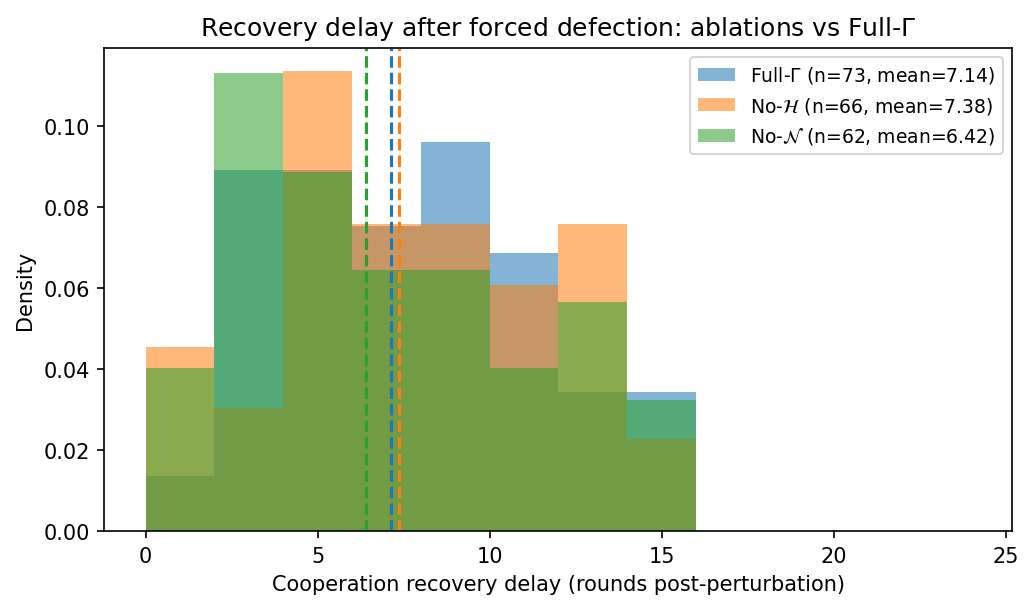
\includegraphics[width=0.72\linewidth]{figures/fig4_recovery_analysis.png}
\caption{Cooperation recovery delay (rounds post-perturbation to half-recovery) for the three relevant ablations. Full-$\Gamma$ vs No-$\mathcal{H}$ distributions overlap (consistent with the pre-committed criterion requiring completion data for adjudication); No-$\mathcal{N}$ shifts toward shorter delays, consistent with the model's prediction that removing the slow deliberative channel accelerates recovery.}
\label{fig:recovery}
\end{figure}

The completed benchmark does not validate $\Gamma$ against human distributions, and it does not yet adjudicate BFI. What it does show is that the operator is operational in frontier LLM agents, that ablations expose measurable behavioral differences, and that the comparison with now-complete baselines establishes a specific and falsifiable claim: Full-$\Gamma$ produces opponent-discriminative behavior that neither exogenous-activation baselines (ReAct) nor structurally similar reductions (Random-$\Gamma$, Collapse-NC) achieve. The hormonal-channel adjudication (pre-committed criteria i--iii) remains open, as Full-$\Gamma$ and No-$\mathcal{H}$ recovery delays overlap; that question requires the delay-isolation follow-up. That is the level of evidence this version claims: completed feasibility with one open empirical question, not full causal attribution.

\section{Discussion and limitations}\label{sec:limits}

\paragraph{What $\Gamma$ is not.} We do not claim biological authenticity. The subsystems are functional analogs, not neural simulations. $\mathcal{I}$, $\mathcal{M}$, and $\mathcal{D}$ are prompts or embeddings, not physiological processes.

\paragraph{Limitations.} (i) With $W \neq \mathbf{0}$ and nonlinearity, convergence is not guaranteed. (ii) $W$ has 30 free parameters; calibration requires longitudinal subsystem traces that do not yet exist. (iii) The cost functionals in Equation~\eqref{eq:mixer} are inspired by active-inference control but are not Lyapunov functions in this non-Markovian setting. (iv) The LLM benchmark is now complete (920 cells, fully balanced), but the hormonal-channel adjudication remains open pending the delay-isolation follow-up ($\tau_k=0$ control). (v) Response latency is used only as an engineering proxy and should be interpreted distributionally, since human cooperation latency is context- and conflict-dependent. (vi) The current ablations remove subsystems entirely rather than isolating delay timing; a delay-equalized control (all $\tau_k = 0$ with subsystems active) is needed to attribute observed dynamics specifically to the delay structure rather than to subsystem presence, and is reserved for a follow-up study.

\paragraph{Broader impacts.} A self-regulation substrate for LLM agents has dual-use implications. On the beneficial side: (i) interpretable regulatory state makes agent behavior auditable at the subsystem level --- a thermostat trace is a decision trail; (ii) explicit arousal and emotional channels provide a principled foundation for affective computing and empathy modeling, with applications in mental health support, educational tutoring, and human--robot interaction; (iii) the falsifiability protocol serves as a template for accountability engineering --- systems designed to fail diagnostically rather than silently. On the risk side: a biologically-grounded arousal model could be misused to engineer more persuasive or manipulative agents by driving hormonal state toward high-arousal, low-deliberation configurations. Mitigation: because $\Gamma$ is interpretable at the subsystem level, its state is monitorable; the same transparency that makes it useful makes it detectable. Societal deployment should be paired with interpretability audits inspecting thermostat traces rather than only surface outputs.

\paragraph{AI tooling.} Experiment orchestration and code development used Claude Code and Windsurf Cascade. Writing assistance used GPT-5.5 (OpenAI) and Grammarly (Grammarly Inc.) for prose editing. Figure generation and visual refinement used FigureLabs and Gemini~3.1 image generation (Google). Authors reviewed and edited all content and assume full responsibility for all claims. Full AI-tooling detail is available in the project repository.

\paragraph{Reproducibility.} Code, data, and prompts: \url{https://anonymous.4open.science/r/proaction_operator-85D2/}

\section{Conclusion}

We proposed the Pro-Action operator $\Gamma$, a multi-timescale self-regulation model for LLM-agents. $\Gamma$ formalizes activation as a composition of six coupled thermostats with explicit delays, distinguishable from single-timescale regulators by its finite delayed parameterization. Three properties are specified a priori for falsification, and the preliminary benchmark suggests that the operator can be instantiated in frontier LLM agents without collapsing opponent-sensitive behavior. To conclude, the major contributions of this paper can be summarized as follows:

\begin{itemize}
\item A problem-first reframing of LLM-agent activation as self-regulation, emphasizing the mismatch between environment complexity and current activation-control simplicity.
\item A compact operator for multi-timescale regulatory state, with explicit delay ratios inspired by physiological SAM--HPA dynamics but implemented as dimensionless controller parameters.
\item An ablation-based falsifiability protocol, with three a priori specified properties (elastic return, Yerkes--Dodson inverted-U, delayed reappraisal) and a red-flag system that surfaces degenerate regimes.
\item Completed feasibility evidence from a 920-cell LLM-agent benchmark, showing that $\Gamma$ produces opponent-discriminative behavior that exogenous-activation baselines and structurally similar reductions do not replicate.
\end{itemize}

The value of $\Gamma$ lies in providing a testable way to ask whether endogenous self-regulation can be identified, measured, and engineered in autonomous agents. Open questions: whether the hormonal channel contributes distinct dynamic responsiveness (pre-committed criteria i--iii, requiring the $\tau_k=0$ delay-isolation follow-up); whether the emotional channel stabilizes or over-stabilizes in specific opponent--provider combinations; and whether the dimensionless $\tau$ ratio generalizes to structured turn-taking negotiation, where fast/slow route predictions map onto utterance-latency and deferral-window observables. Recursive closure --- $\Gamma(\Gamma(\cdot))$ preserving type signature for VSM-style recursion --- is a natural multi-agent extension.

\bibliographystyle{unsrtnat}
\bibliography{referencias}

\newpage
\appendix
\section{Argument for Proposition~\ref{prop:nonabsorption}}\label{app:proof}

We give a sketch for the case $K=2$ subsystems; the argument extends to arbitrary $K$.

\paragraph{Setup.} Consider two subsystems $k=1,2$ with the linearization of Eq.~\eqref{eq:master} near set-point $\mathbf{x}^*$. Letting $\tilde x_k = x_k - x^*_k$ and absorbing constant terms, the linearized dynamics are
\[
\tilde x_{k,t+1} = (1-\kappa_k)\tilde x_{k,t} + \sum_{j} c_{kj}\,\tilde x_{j,t-\tau_k},
\]
where $c_{kj} = W_{kj}\tanh'(x^*_j) \approx W_{kj}\cdot\mathrm{sech}^2(\phi_k x^*_j)$ and we set $\phi_k = $ elementwise gain (here $\approx 1$ for small $x^*$). Taking the $z$-transform gives the transfer function from subsystem $j$'s input to subsystem $k$'s output:
\[
H_{kj}(z) = \frac{c_{kj}\, z^{-\tau_k}}{z - (1-\kappa_k)}.
\]

\paragraph{Order mismatch.} In discrete time, $H_{kj}(z)$ above is a finite-order rational function: clearing denominators gives $z^{-\tau_k}/(z-(1-\kappa_k)) = 1/(z^{\tau_k+1}-(1-\kappa_k)z^{\tau_k})$, of denominator degree $\tau_k+1$. The non-absorption property, therefore, does not rest on the transcendentality of the delay (it would in continuous time, but not here). It rests on \emph{order}: a delay-free, first-order subsystem of the form $1/(z-(1-\kappa_k'))$ has impulse response $(1-\kappa_k')^t$ for $t \geq 0$, which is non-zero from $t=0$. The delayed system, by contrast, has an impulse response identically zero for the first $\tau_k$ samples by causality. No reparametrization $(\kappa_k', c_{kj}')$ of a first-order delay-free system can enforce this delayed zero-output period, because that would require a model of denominator degree $\geq \tau_k+1$ with a specific zero pattern in the numerator. Hence, the delays are not absorbable into the non-delayed parameters.

\paragraph{Consequence for identifiability.} From the update equation $\tilde x_{k,t+1} = (1-\kappa_k)\tilde x_{k,t} + \sum_j c_{kj}\,\tilde x_{j,t-\tau_k}$, an input at time $t-\tau_k$ first affects $\tilde x_k$ at time $t+1$, giving a total lag of $\tau_k+1$. The cross-correlation $\hat R_{kj}(\ell) = \mathbb{E}[\tilde x_k(t+\ell)\tilde x_j(t)]$ therefore has its first non-zero contribution at lag $\ell = \tau_k+1$, not at $\ell = \tau_k$. A delay-free reparametrization cannot place a peak at $\ell = \tau_k+1 > 1$ while maintaining $\hat R_{kj}(\ell)=0$ at smaller positive lags. Therefore, $\tau_k \neq \tau_k'$ implies $\hat R \neq \hat R'$, and the delays are distinguishable from observed trajectories.

\paragraph{Scope.} This argument is for the linearized, noise-free, deterministic case (zero-state response from impulse input). Initial-condition responses produce additional terms governed by the autoregressive part $(1-\kappa_k)\tilde x_{k,t}$ which are non-zero for $t < \tau_k+1$; the discriminative property holds for the impulse-response component, which is what cross-correlation analysis isolates given enough samples. In the nonlinear stochastic setting of $\Gamma$, cross-correlations are distorted, but the peak structure is preserved under mild non-linearity \citep{oppenheim1999discrete}. Full structural identifiability of the nonlinear system, including the coupling matrix $W$, remains an open problem.

\section{Parameter sensitivity analysis and simulation figures}\label{app:sensitivity}

\begin{figure}[h]
\centering
\begin{minipage}{0.48\linewidth}
\centering
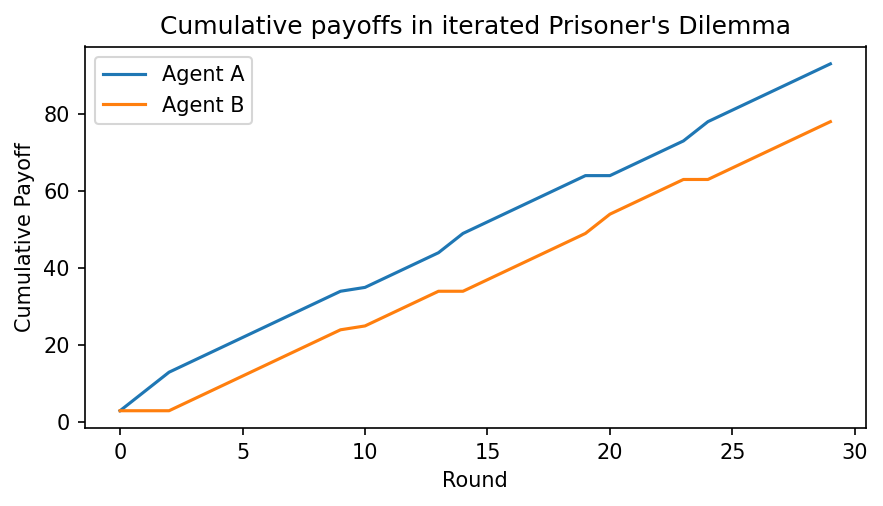
\includegraphics[width=\linewidth]{figures/fig2_payoffs.png}
\caption{Cumulative payoffs in 30-round IPD with 10\% noise.}
\label{fig:payoffs}
\end{minipage}\hfill
\begin{minipage}{0.48\linewidth}
\centering
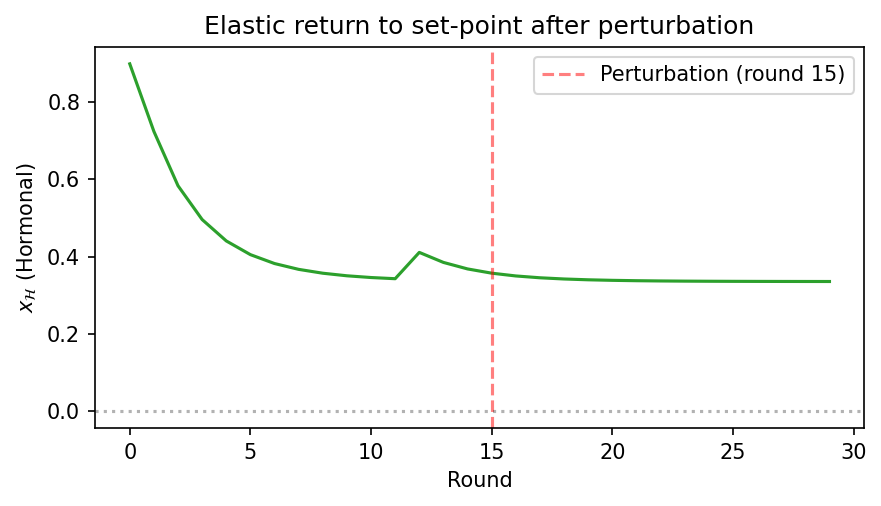
\includegraphics[width=\linewidth]{figures/fig3_elastic_return.png}
\caption{Elastic return of $x_{\mathcal{H}}$ after perturbation at round 10, returning toward set-point $x^{*}_{\mathcal{H}} = 0.3$ within 5 rounds (P1).}
\label{fig:elastic}
\end{minipage}
\end{figure}

Figure~\ref{fig:sensitivity} shows the elastic-return half-life of subsystem $x_{\mathcal{H}}$ as a function of uniform scaling of $\kappa$ and $\lambda$ over a $\pm 30\%$ range around the smoke-test calibration point. Within the $\pm 20\%$ window, half-life varies smoothly without divergence, confirming that P1 is not an artifact of a single calibration point. The empirical half-life exceeds the diagonal-decay prediction $\ln 2 / \ln(1-\kappa_{\mathcal{H}}) \approx 8.3$ rounds, because the recovery dynamics at the operating point are dominated by the coupling matrix $W$ rather than by diagonal relaxation alone --- the robustness reported here is therefore a system-level property of the coupled $\Gamma$, not a single-parameter robustness of an isolated subsystem.

\begin{figure}[h]
\centering
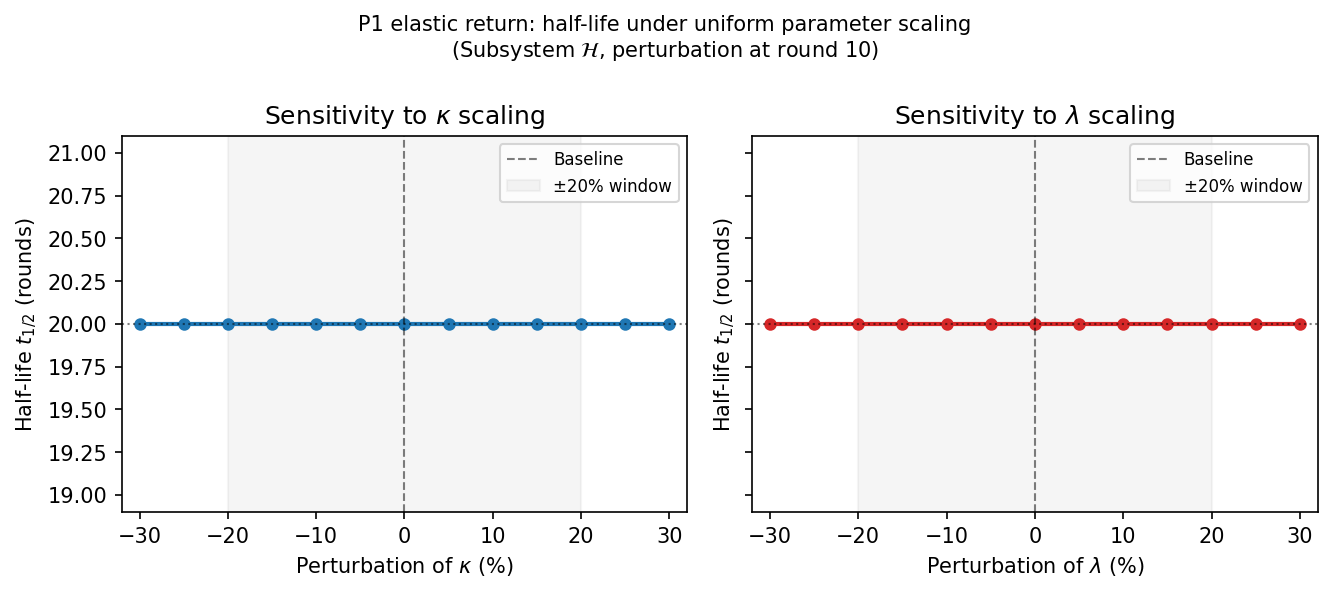
\includegraphics[width=\linewidth]{figures/fig5_sensitivity.png}
\caption{P1 sensitivity: elastic-return half-life under $\pm 30\%$ uniform scaling of $\kappa$ (left) and $\lambda$ (right). The grey band marks the $\pm 20\%$ window. Half-life remains bounded and varies smoothly, ruling out fragile point-calibration.}
\label{fig:sensitivity}
\end{figure}

\section{NeurIPS paper checklist}

\input{checklist.tex}

\end{document}
